\documentclass{anstrans}
% % % % % % % % % % % % % % % % % % % % % % % % % % % % % % % % % % % % % % % % % % % % % % % % % % % % % % % % % % % % %
\title{Decay Heat Measurements and Calculations}
\author{Kristina Yancey}

\institute{Texas A\&M University, 3133 TAMU, College Station, TX}

\email{kristina.yancey@gmail.com}

%%%% packages and definitions 
\usepackage{graphicx} % allows inclusion of graphics
\usepackage{booktabs} % nice rules (thick lines) for tables
\usepackage{microtype} % improves typography for PDF 

\begin{document}

\section{Introduction}
After a fission event, the decay heat is one of the most important pieces of information about a nuclear material. This is especially true in the case of spent fuel because it characterizes the cooling requirements to maintain safety. In the case of an accident, the decay heat must be accounted for to prevent the coolant from boiling away and exposing the fuel. In the case of storage, the decay heat determines the length of time that an assembly has to be kept in the spent fuel pool and defines the thermal needs for any dry cask design. For this reason, it is important to accurately measure and predict the amount of heat that a spent fuel assembly produces.

% % % % % % % % % % % % % % % % % % % % % % % % % % % % % % % % % % % % % % % % % % % % % % % % % % % % % % % % % % % % % %
\section{Decay Heat Measurement Methods \& Techniques}
Since decay heat travels beyond its microscopic region, nondestructive means can be used to evaluate the fuel. There are two primary measurement techniques used to assess decay heat:
\begin{enumerate}
\item Calorimetry
\item Spectroscopy
\end{enumerate}
Calorimetry allows for the total decay heat to be measured, and spectroscopy distinguishes the different levels of energy released through each beta or gamma decay \cite{Tobi1980}.

To quantify the heat production, the general calorimeter consists of a container, a temperature sensor, and a heat sink, as shown in Fig.~\ref{fig:brac1}. The measurement produced with this setup is independent of the source material and matrix type, so it can be used with any heat-producing substance \cite{Brac2007}. Since spent fuel contains a large number of long-lived nuclides, the time scale to produce a noticeable change is usually weeks or months. The advantage of this technique is that it is very precise and nearly bias free, which can be determined during calibration. At the most general level, the heat is calculated using Eq.~\eqref{eq:heat}.
\begin{equation} \label{eq:heat}
\frac{dQ}{dt} = k (T_{cal} - T_{env})
\end{equation}
Here, $Q$ represents the heat produced, $t$ represents the time, $k$ is the thermal conductivity, $T_{cal}$ is the temperature inside the calorimeter, and $T_{env}$ is the temperature of the surrounding environment.
\begin{figure}[ht]
 \centering
 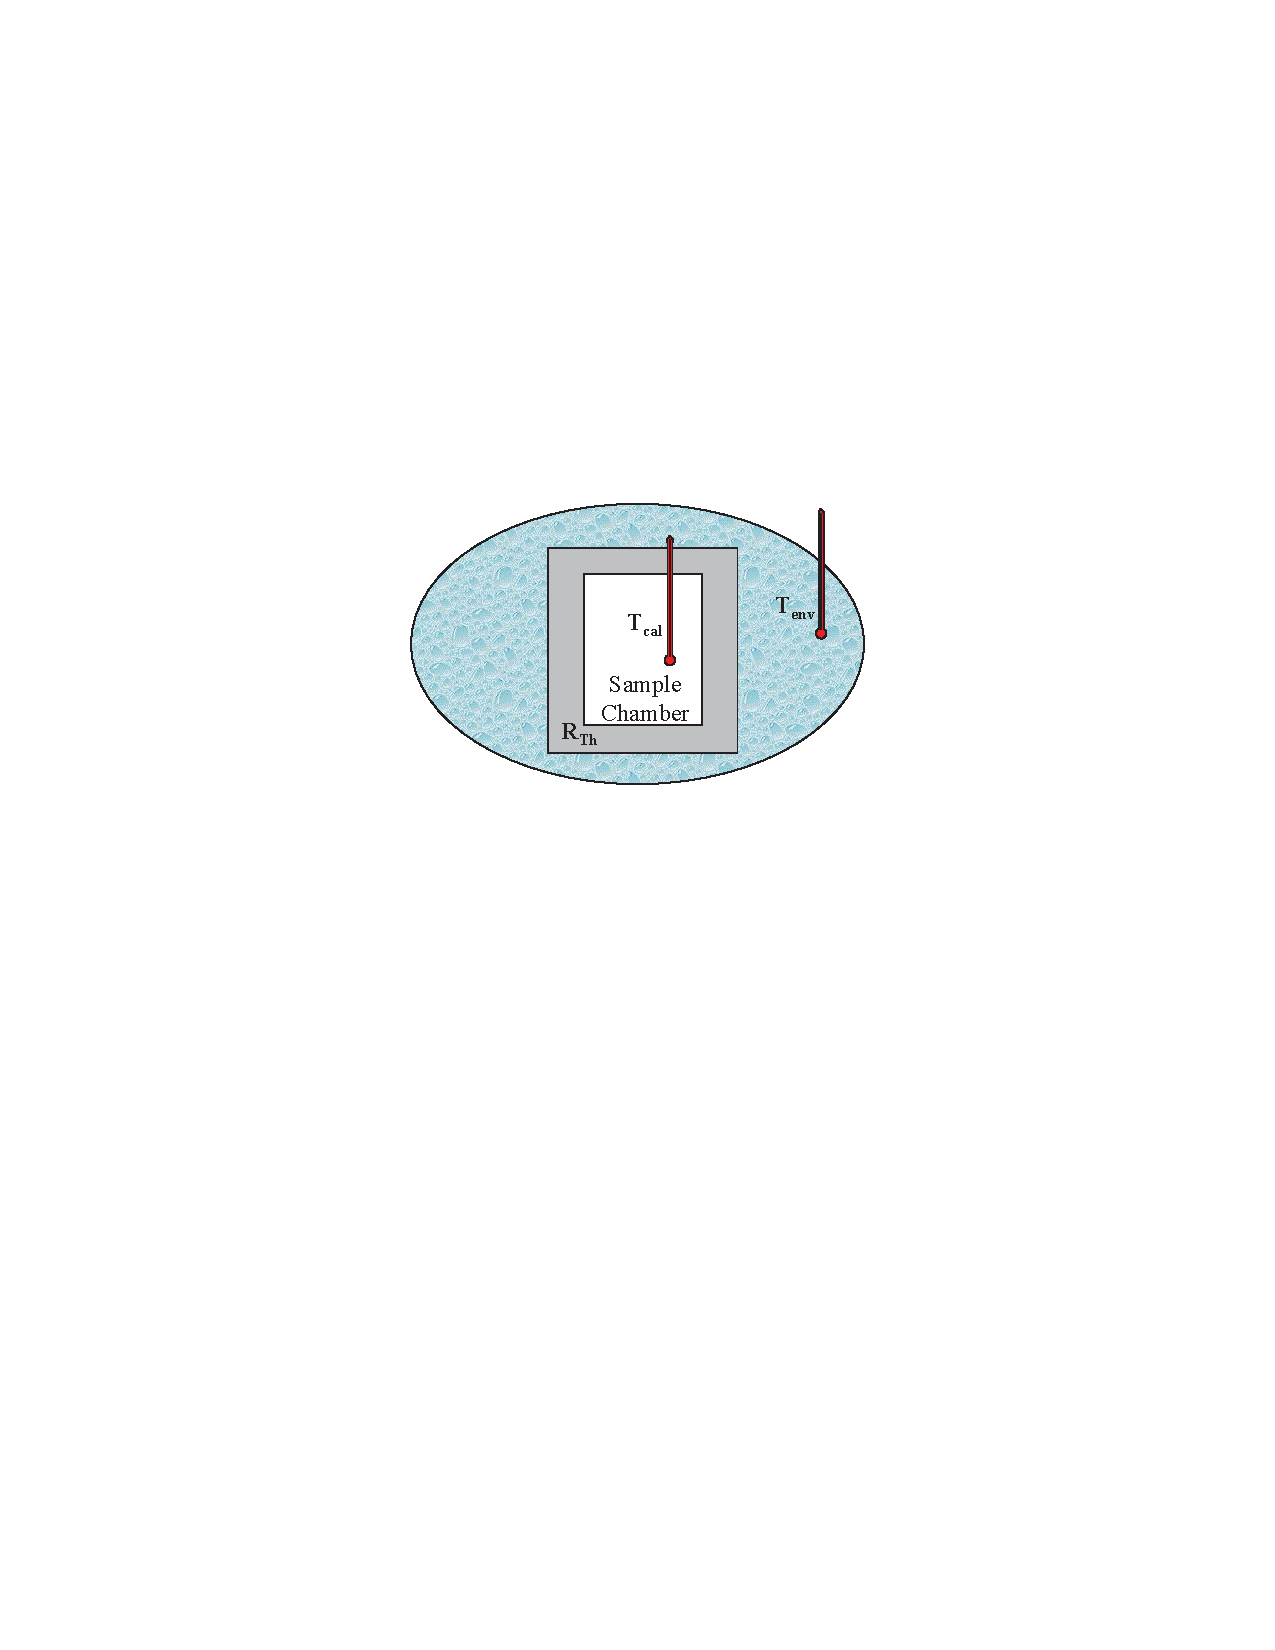
\includegraphics{Pictures/bracken1}
 \caption{Schematic of minimum components necessary to perform a heat measurement. Borrowed from \cite{Brac2007}.}
 \label{fig:brac1}
\end{figure}

While Geiger counters and ionization chambers were used in early measurements to complement calorimetry data, scintillation spectroscopy is the predominant alternative used today \cite{Tobi1980}. Scintillators convert the kinetic energy of charged particles into light through induced luminescence of a crystal \cite{Knol2000}. The decay time of the luminescence should be short enough that a fast signal pulse can be generated in the photomultiplier tubes and photodiodes. While many crystals are available, the most popular in gamma-ray spectroscopy is NaI(Tl) due to its "extremely good light yield, excellent linearity, and the high atomic number of its iodine constituent" \cite{Knol2000}. Figure~\ref{fig:will1} shows an example of a typical spectrum from a spent fuel assembly of a Pressurized Water Reactor (PWR). Spectra, such as this example, are used in combination with knowledge of photon interactions to determine the most prominent energies released during decay. Dividing the number of counts registered by the detection time gives the intensity of each peak. In addition to characterizing the decay heat, this information can be used to determine the burnup of the fuel \cite{Will2006}. 
\begin{figure}[ht]
 \centering
 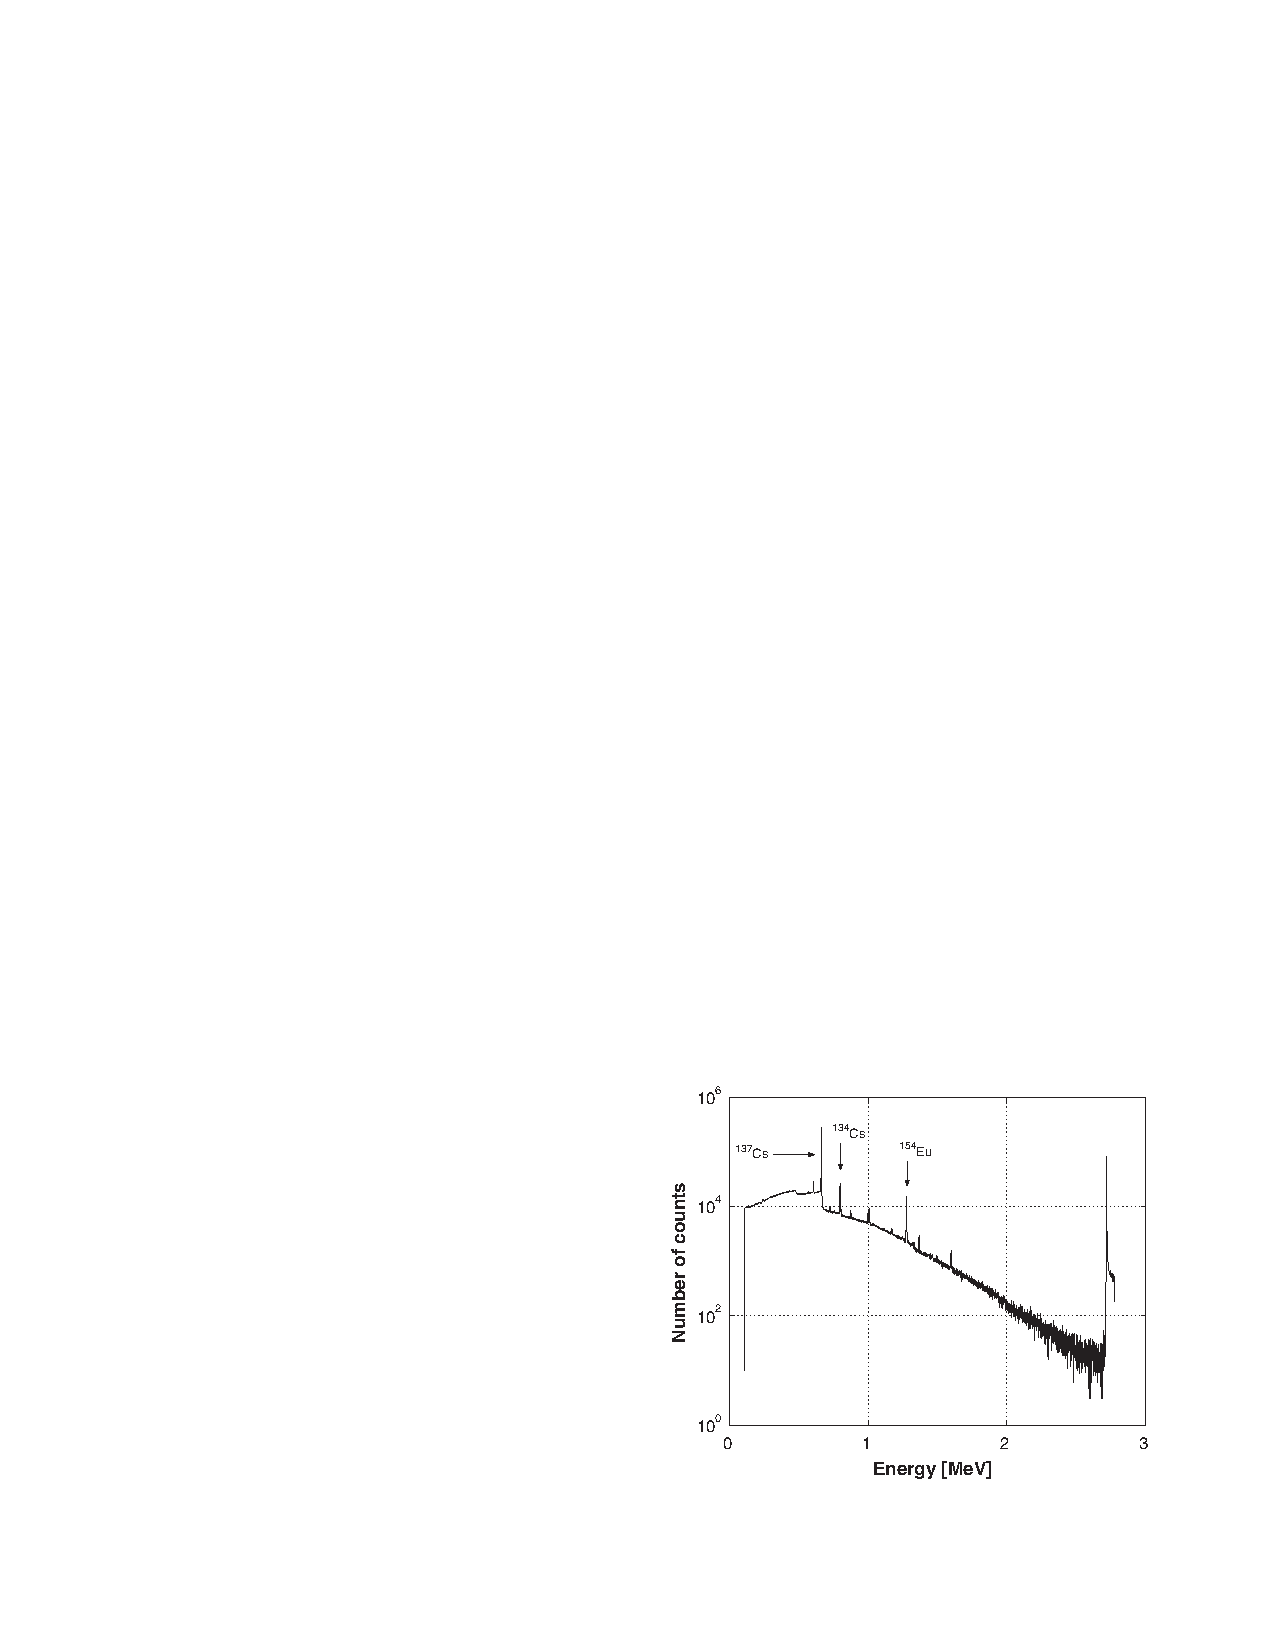
\includegraphics{Pictures/willman1}
 \caption{A typical spectrum of one corner of a fuel assembly with a burnup of 47 GWd/MTU and a cooling time of 12 years. The peak around 2.7 MeV is the pulser peak used for dead-time correction \cite{Will2006}.}
 \label{fig:will1}
\end{figure}

% % % % % % % % % % % % % % % % % % % % % % % % % % % % % % % % % % % % % % % % % % % % % % % % % % % % % % % % % % % % % %
\section{Predictive Equations of Spent Fuel Decay Heat}
While decay heat measurements provide a "true picture" of the decay heat in spent fuel, predictions of decay heat are often needed to augment the data. Examples of this include when a dry cask is designed to last far longer than the time frame of experimental measurements or when a reactor designer is considering a new fuel type that does not necessarily fit inside the parameters of the spent fuel already studied. 

There are two main methods of calculating the decay heat after a fission event:
\begin{enumerate}
\item Statistical Models
\item Summation Calculations
\end{enumerate}
The first method was initially proposed by Way and Wigner in 1948 and treated the fission products as a statistical assembly \cite{Way1948}. The authors developed empirical relations for the nuclide distributions over time and for the relationship between the half-life to the maximum energy of a beta decay. It was recognized that the method was incomplete and was only valid when many nuclides were contributing to activity shortly after fission. The statistical method was still considered to be useful because it agreed reasonably well with experimental data, and decay data was only available for less than 100 nuclides around that time \cite{Tobi1980}. 

Summation calculations gradually replaced statistical models as evaluated data continued to improve, including data for 724 nuclides by 1978 \cite{Tobi1980} and over 3800 materials today \cite{Chad2011}. The basic summation formulation is shown in Eq.~\eqref{eq:summation} \cite{Nich2002}.
\begin{equation} \label{eq:summation} 
H(t) = \sum_{i=1}^{M} (E^i_\alpha + E^i_\beta + E^i_\gamma)\lambda^T_i N_i(t)
\end{equation}
Here, $H(t)$ represents the total decay heat over time $t$, $i$ represents each unstable nuclide, $M$ represents the total number of nuclides, $E^i$ represents the average energy released by an alpha, beta, or gamma decay, $\lambda$ represents the decay constants, and $N_i(t)$ is the number of atoms of nuclide $i$ present in the system. Given the fidelity of evaluated data, this equation can be used to predict the decay heat for thousands of years.

Despite the advances in summation calculations, other methods are available to calculate decay heat. The American National Standard for Decay Heat Power in Light Water Reactors (LWRs) provides a simple procedure to calculate decay heat in the same vain as earlier statistical models \cite{ansi2005}. The purpose of the standard is to determine shutdown decay heat power and its uncertainty for LWRs and therefore is not reasonably extended to other systems. It presents two methods for the calculation: one based on the decay heat following an instantaneous burst of fission and one based on the decay heat from fission products after an infinitely long operating period. Neither method accounts for neutron capture by fission products, so the standard also includes a corrective multiplying factor that gives an upper bound for this effect. The decay heat power is presented in tables with units of (MeV/s)/fission, and formulas are presented to convert the tabulated data into physically relevant values. The standard presents the decay heat power for \textsuperscript{239}U and \textsuperscript{239}Np separately.

\begin{figure}[ht]
 \centering
 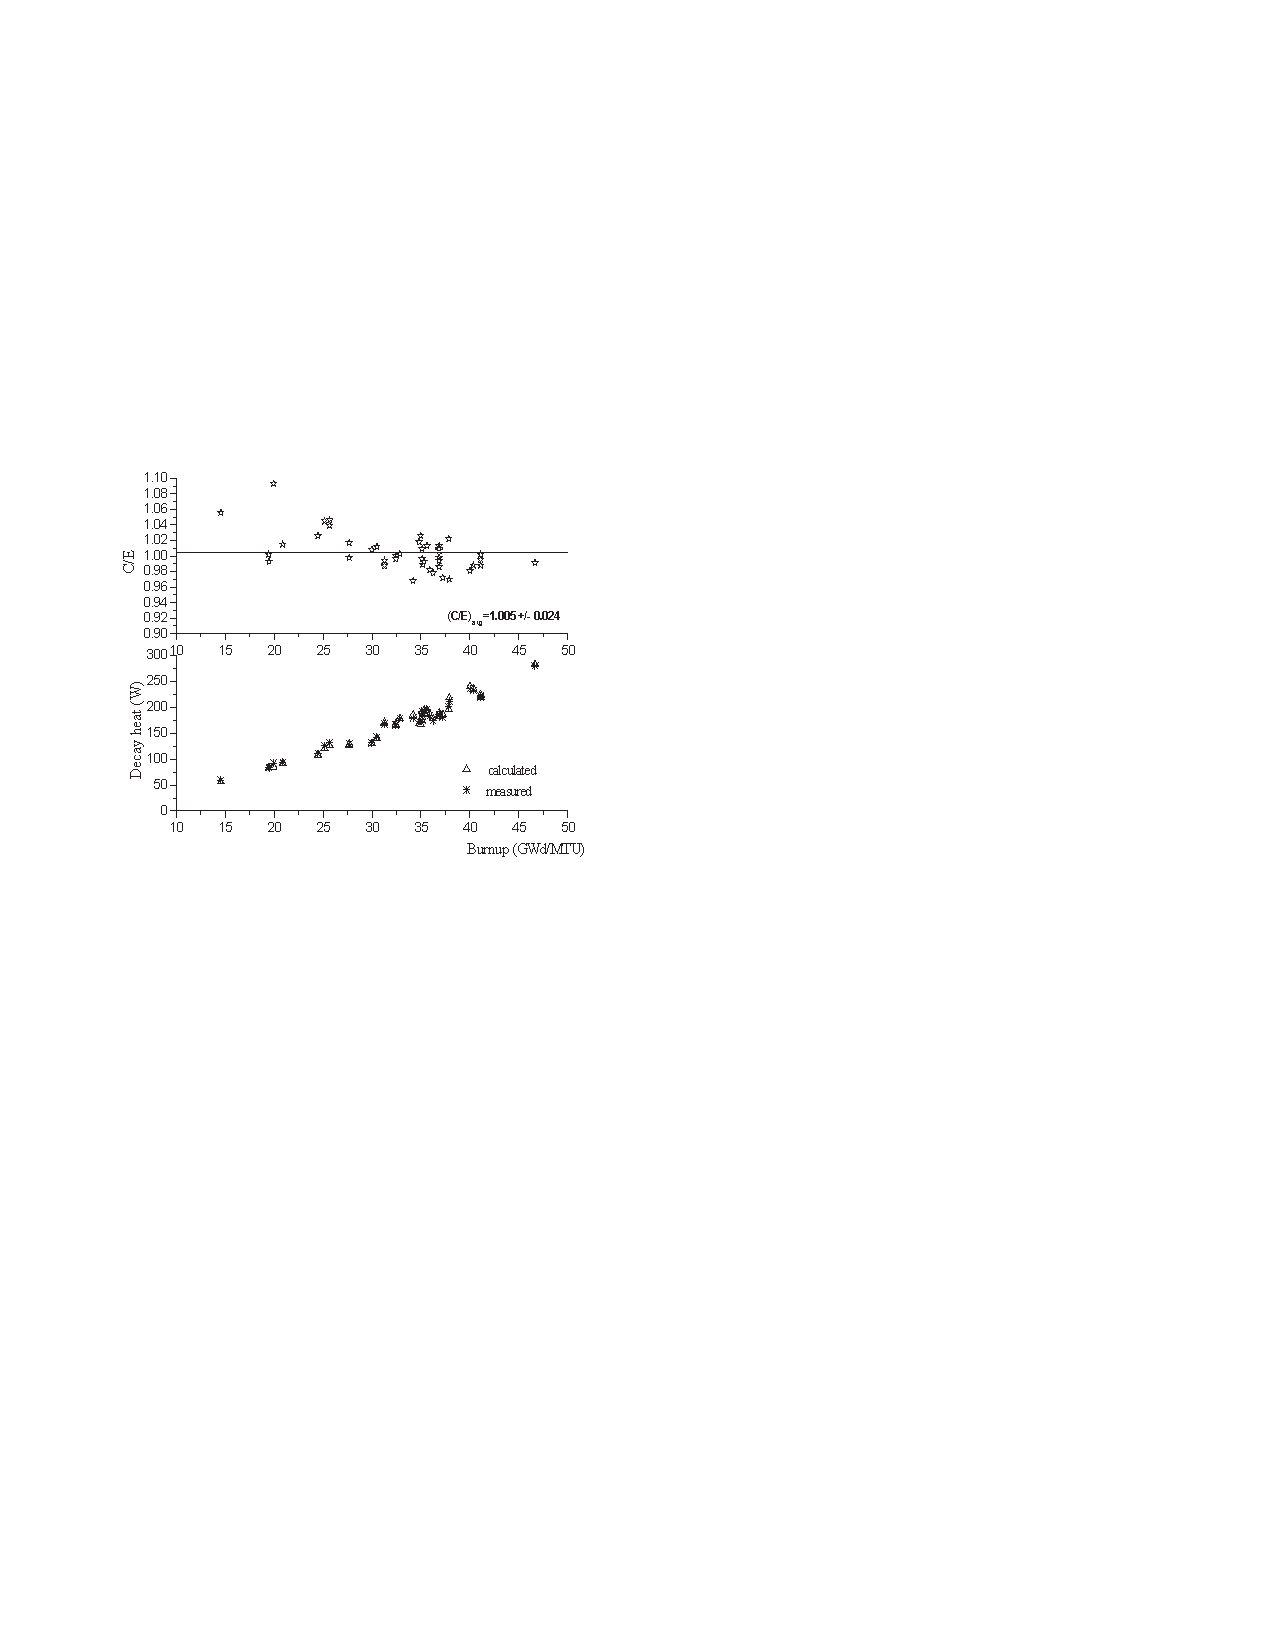
\includegraphics{Pictures/ilas1}
 \caption{Comparison of measured and calculated decay heat values. Borrowed from \cite{Ilas2006}.}
 \label{fig:ilas1}
\end{figure}

Hybrid models have also been developed that seek to marry macroscopic measurements with summation calculations. One such method is based on the idea that the decay heat power is a linear function of the fission yield \cite{Oyam2001}. Since the fission yield is a gradual and relatively regular function of atomic mass and proton number, the study proposed that any yield could be approximated by a linear combination of fission yield vectors of other systems, as in Eq.~\eqref{eq:yield}.
\begin{equation} \label{eq:yield}
y = a_1 y_1 + a_2 y_2 + a_3 y_3 + a_4 y_4 + y_R
\end{equation}
Here, $y$ denotes the fission yield vector, the subscripts 1 through 4 denote the other fissioning systems, and $y_R$ denotes the residual term. The first four yields come from macroscopic measurements, and residual term must be found with summation calculations. The values of the coefficients $a_1$ to $a_4$ are chosen to minimize the residual term. This method was shown to be reliable before 4000 s of decay and unreliable after that time due to some unknown reason.

% % % % % % % % % % % % % % % % % % % % % % % % % % % % % % % % % % % % % % % % % %
\section{Current Developments}
Although the state-of-the-art measurements and calculations have reached a high level of fidelity, improvements continue to be made. Nuclear reactors have seen a steady increase in fuel burnup, due both to improved designs and in-core fuel cycle optimizations. In the early 2000's, reactor models began to move beyond the existing validated domains, and efforts were undertaken to obtain new measurements of the higher burnup fuel. The Central Interim Storage Facility (CLAB) in Sweden completed one such study, performing calorimeter measurements of full-length LWR assemblies over a large burnup range, up to 47 GWd/MTU \cite{Ilas2006}. These measurements were then used at Oak Ridge National Laboratory (ORNL) to validate decay heat calculations performed by the SCALE computer system.

Figure~\ref{fig:ilas1} presents the results of this validation, focusing only on Boiling Water Reactor (BWR) data. A set of 45 measurements were available in this category, and 2-D models were performed to simulate each data point. The average of the calculated-to-experimental (C/E) ratio was 1.005 with a standard deviation of 2.4\%. The top portion of Fig.~\ref{fig:ilas1} presents this ratio as a function of burnup. The figure validates the usage of SCALE for decay calculations of higher burnup BWR spent fuel. This study was later augmented with further measurements from GE-Morris and the Hanford Engineering Development Laboratory, and the code was validated for both BWR and PWR spent fuel decay heat predictions, showing that the calculated values generally lie within the uncertainty of the decay heat measurements \cite{Gaul2010}.

Decay heat measurements themselves have seen improvements during the past several years. In 1977, the idea of the "pandemonium effect" was put forth \cite{Hard1977}. The basis of the idea was the common assumption that any beta decay that did not produce a noticeable gamma peak on a spectrum created by a high-resolution detector must not be a significant part of the nuclide's decay scheme. The authors argued that this is only a valid assumption if the beta decay energy was low, but for beta decays with high energy and many available final states, the gamma spectrum might still be unresolved, analogous to neutron resonance regions. They demonstrated the possibility using a fictional nucleus named "Pandemonium," which was modeled using broad statistical principles of nuclear excitation and decay. They chose $A$=145 and $Z$=64 to compare their results to measurements of \textsuperscript{145}Gd. Their analysis suggested that approximately 20\% of its gamma-ray intensity was not even recognized or included in the decay scheme.

A discrepancy was indeed noticed from 300 to 3000 s after a fission burst between decay heat benchmark data, from full-absorption calorimetry measurements, and summation calculations, based on decay data from spectroscopic measurements.  A number of possible explanations were suggested, including the underestimation of certain half-lives and fission yields, but the missing beta decay strength was highlighted as the simplest answer \cite{Yosh1999}. Based on this work, further studies were completed that identified the highest priority fission products to be resolved: \textsuperscript{102,104,105,106,107}Tc, \textsuperscript{105}Mo, and \textsuperscript{101}Nb \cite{Algo2014}.

A careful procedure was setup to eliminate the pandemonium effect in new measurements of these fission products. A team at the Ion Guide Isotope Separator On-Line (IGISOL) facility at the University of Jyv\"{a}skyl\"{a} combined a total absorption gamma spectometer (TAGS) with a Penning trap for the experiment \cite{Algo2014}. The Penning trap guaranteed the purity of the fission product samples, and new mean gamma and beta decay energies were found. Figure~\ref{fig:algo1} shows the improvement in the summation calculation after inclusion of the TAGS data. 
\begin{figure}[ht]
 \centering
 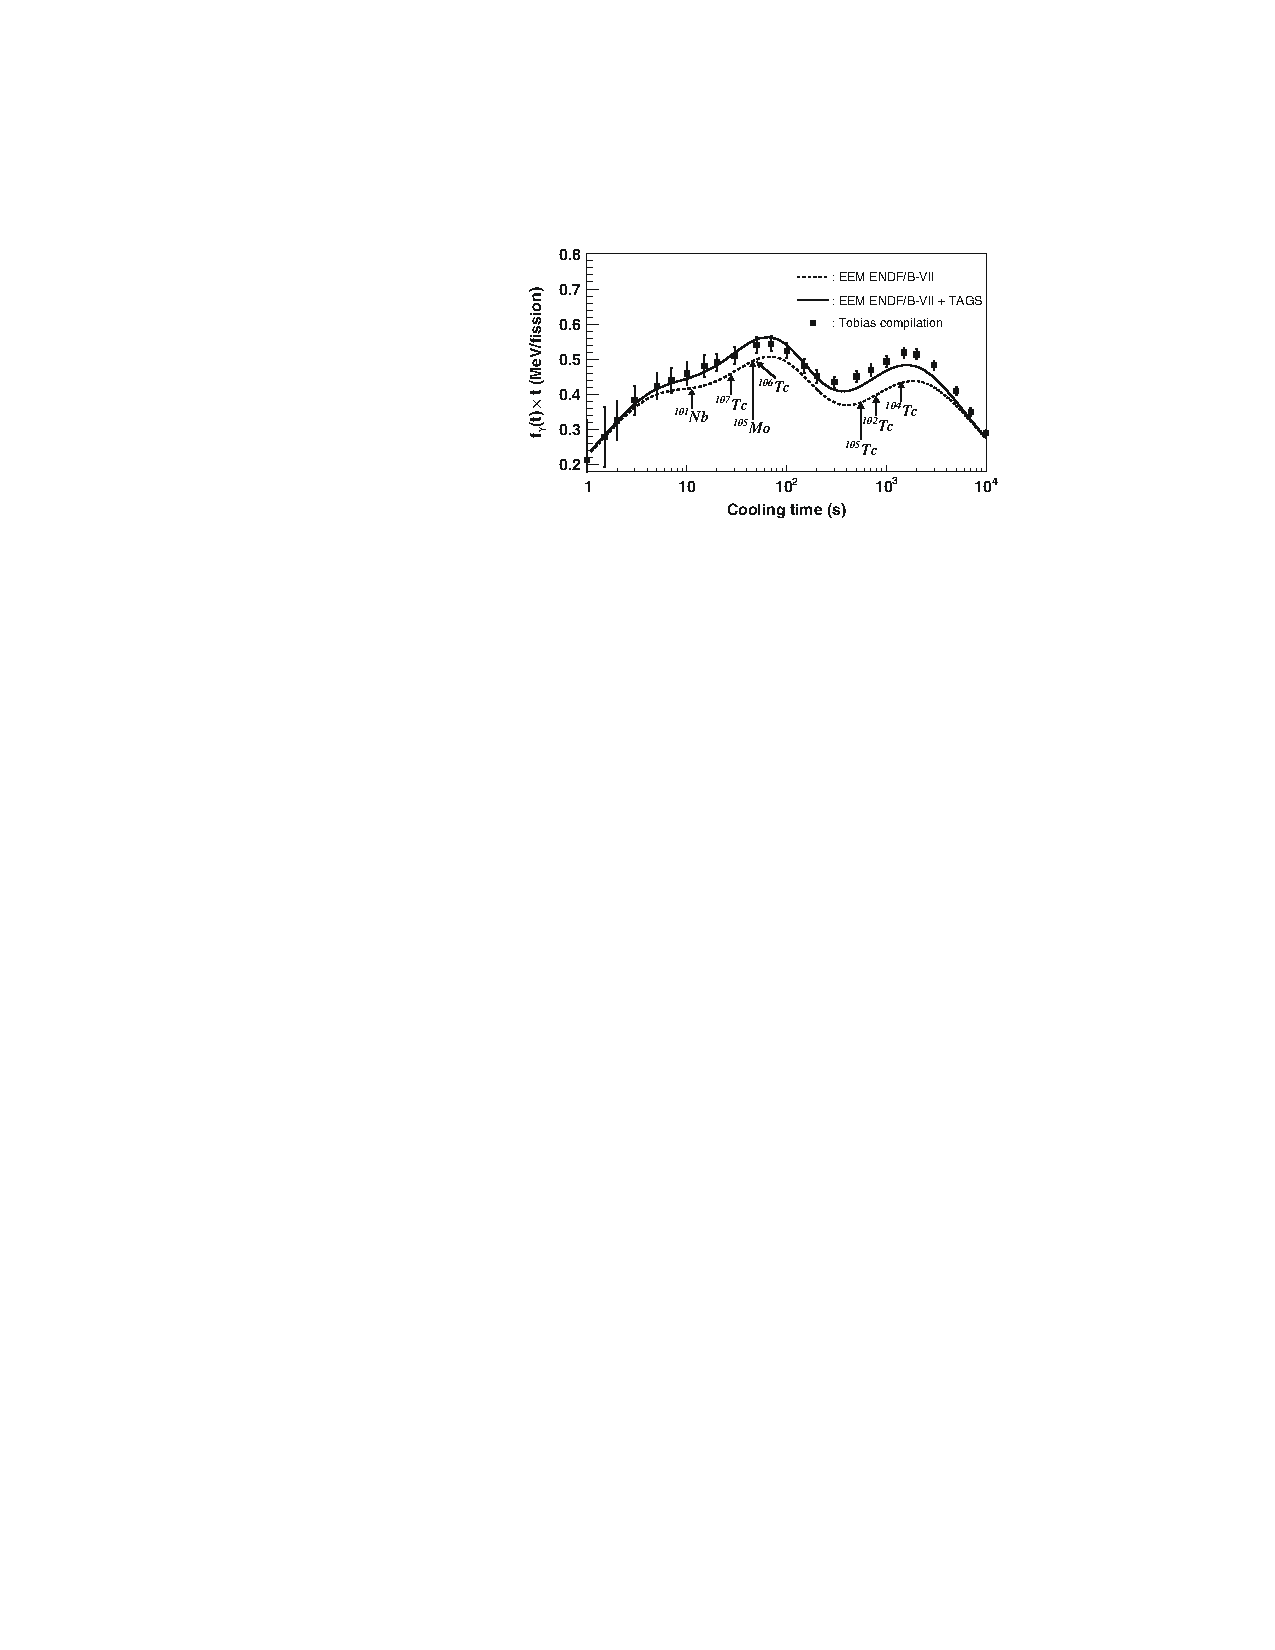
\includegraphics{Pictures/algora1}
 \caption{Comparison of the calculated electromagnetic decay heat component for \textsuperscript{239}Pu before and after the inclusion of measurements with the data of Tobias et al \cite{Tobi1989}. The time of the peak contribution of each of the studied isotopes is marked with arrows. Borrowed from \cite{Algo2014}.}
 \label{fig:algo1}
\end{figure}

\begin{figure}[ht]
 \centering
 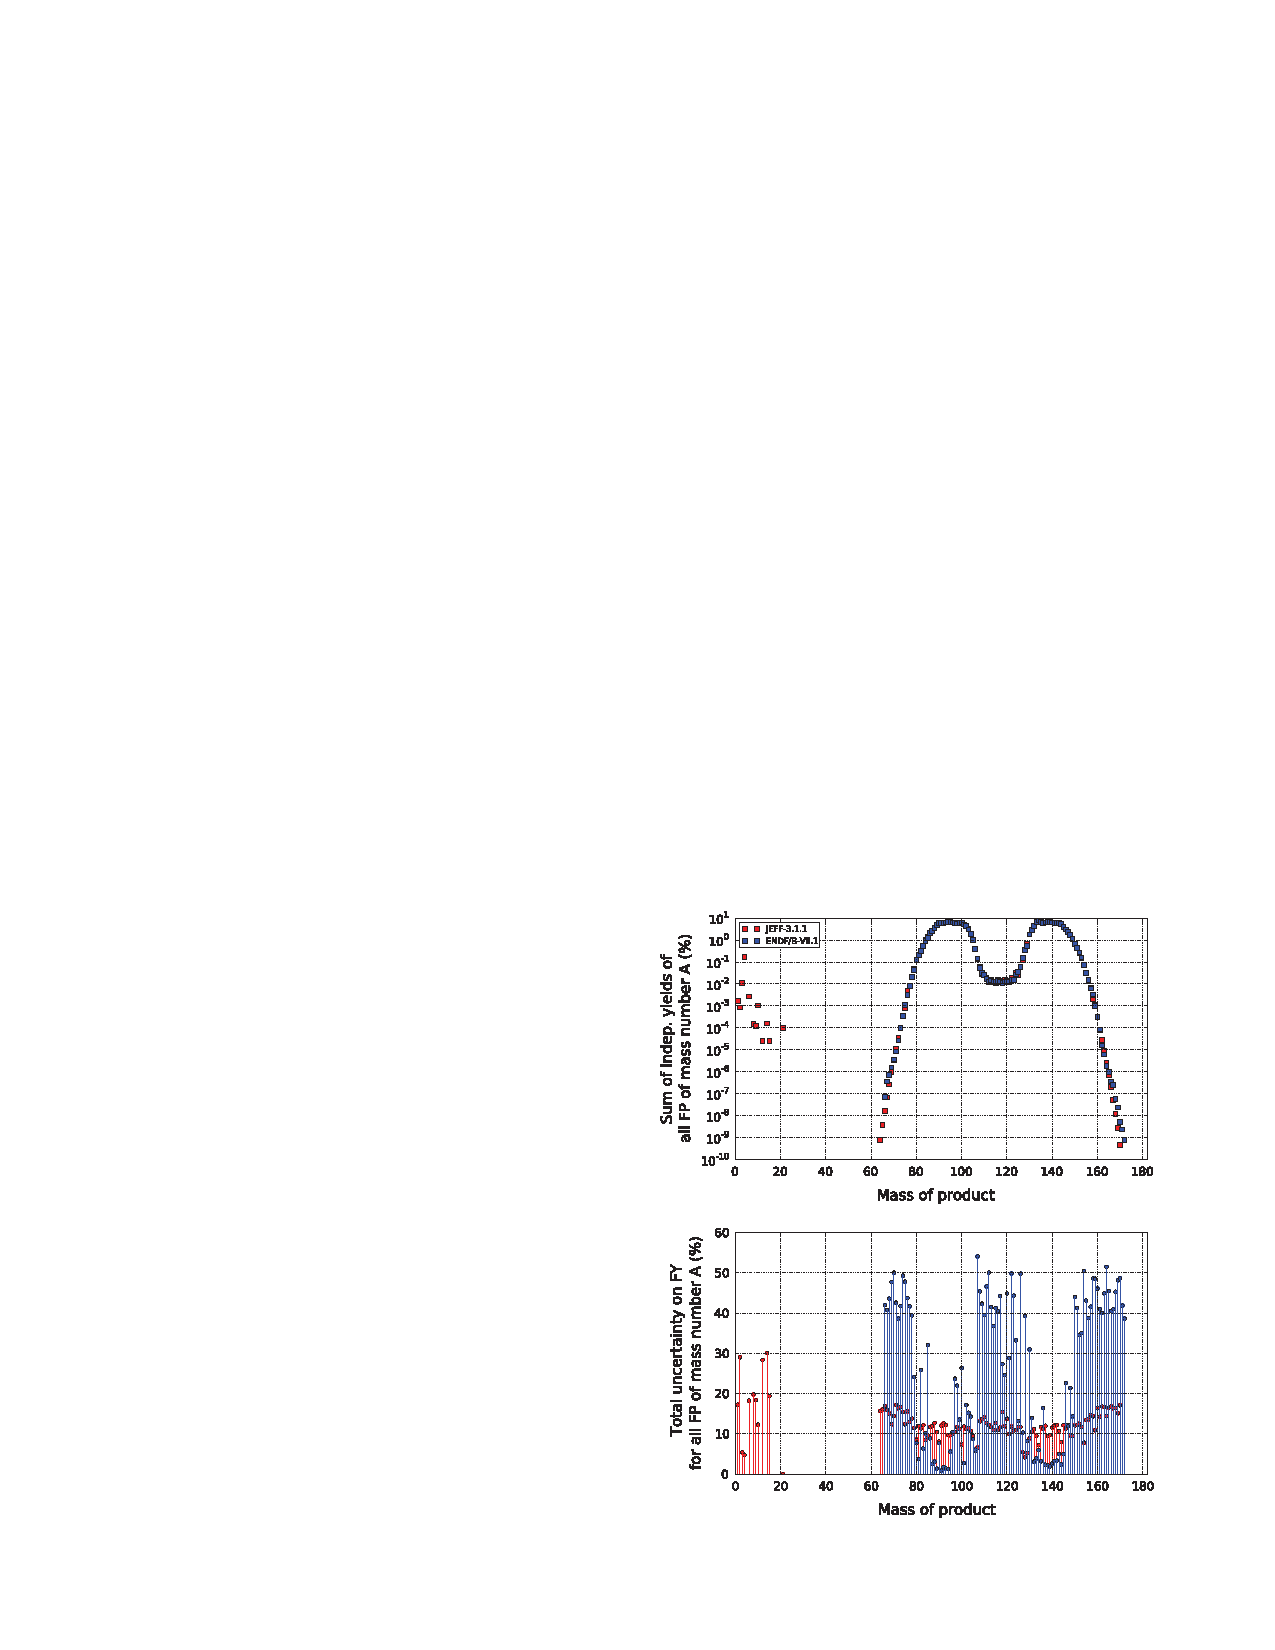
\includegraphics{Pictures/fiorito1}
 \caption{Mass-yields distribution and uncertainties for \textsuperscript{235}U thermal fission products from ENDF/B-VII.1 and JEFF-3.1.2 libraries. Borrowed from \cite{Fior2014}.}
 \label{fig:fior1}
\end{figure}
Simultaneously, improvements are being seen in fission yield uncertainty quantification, which directly relates to decay heat uncertainties. Evaluated data, such as ENDF/B and JEFF, supply fission yields and their standard deviations, but currently they do not supply correlations between fission yields. This has been highlighted as an area for improvement by the Working Party on International Nuclear Data Evaluation Co-operation \cite{Fior2014}. Figure~\ref{fig:fior1} shows general agreement between ENDF/B-VII.1 and JEFF-3.12 in their mass fission yields (MFYs), the sum of the independent fission yields of all fission products with mass number A. The biggest difference between the two is that JEFF-3.1.2 also includes ternary fission products, which are neglected by ENDF/B-VII.1. Conversely, the bottom graph of Fig.~\ref{fig:fior1} shows large differences in uncertainty. ENDF/B-VII.1 assumes larger values of uncertainty for smaller fission yields and smaller values for bigger yields, whereas uncertainties in JEFF-3.1.2 are more evenly distributed. Since the mass fission yields are sums of the independent fission yields, both sets of uncertainty were found through simple propagation, assuming no correlation. 

Within the past couple of years, a few different strategies have been proposed to account for correlations between fission yields: perturbation theory, Monte Carlo parameter perturbation, and the Bayesian/general least-squares (GLS) method \cite{Fior2014}. In Fiorito et al., the Bayesian/GLS method was used to create the covariance matrix for the fission yields, and then full simulations of \textsuperscript{235}U thermal fission were performed using both evaluated data sets to show the improvement in uncertainty quantification. This comparison is shown in Fig.~\ref{fig:fior2}, along with the uncertainty values from \cite{Tobi1989}. Including the covariance matrix in the uncertainty quantification significantly reduces the total uncertainty of the fission product decay heat (FPDH). Not only does this increase the precision of the results, but it also improves the accuracy of nuclides with very low capture cross sections that are critical for depletion problems, such as \textsuperscript{148}Nd.
\begin{figure}[ht]
 \centering
 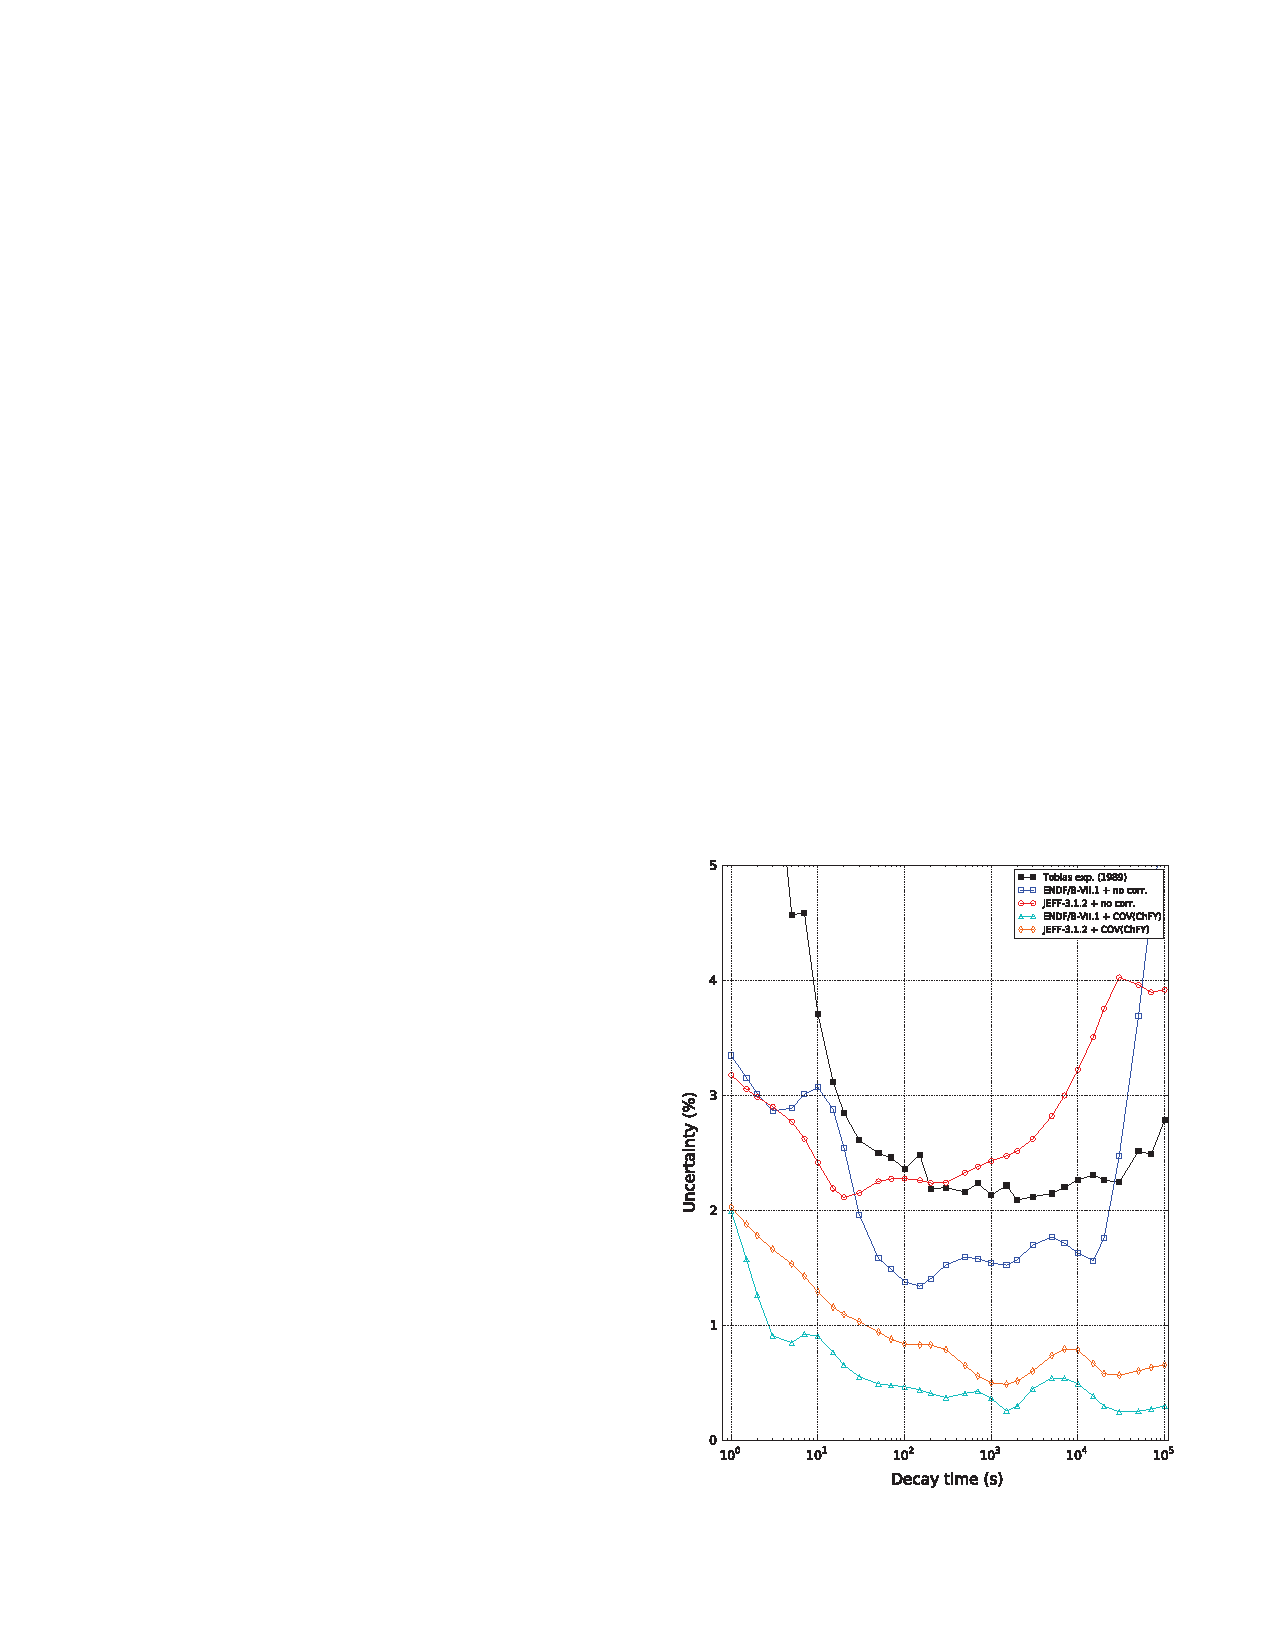
\includegraphics{Pictures/fiorito2}
 \caption{Comparison of uncertainties on thermal FPDH for \textsuperscript{235}U calculated with both JEFF-3.1.2 and ENDF/B-VII.1. Borrowed from \cite{Fior2014}.}
 \label{fig:fior2}
\end{figure}

% % % % % % % % % % % % % % % % % % % % % % % % % % % % % % % % % % % % % % % % % %
\section{Conclusions}
State-of-the-art decay heat measurements and calculations have reached a high level of fidelity. Still, there is room for improvement. As burnup continues to increase, and as accident tolerant fuels are incorporated into the fuel cycle, it will be important to expand the domain of experimental data. It will also be advantageous to perform more careful experiments, such as TAGS, to improve the accuracy of fission product decay heat and to refine the uncertainty quantification of fission yields and beyond. This will help to decrease the burden of redundant safety margins in dry cask design and will aid in the optimization of spent fuel storage.

\bibliographystyle{ans}
\bibliography{bibliography678}
\end{document}